\chapter{Modèles sur réseaux}
    \label{chap-sos}

Comme indiqué dans l'équation \ref{renormalisation},  le champ $\phi(\mx,t)$ est un champ moyenné sur le temps et l'espace à cause de la précision de nos appareils de mesure. Si par exemple le champ $\phi$ représente une densité de particules, alors au niveau le plus fondamental, le champ est charactérisé par
\begin{align}
    \phi(\mx,t) = \frac{1}{V} \sum_i \delta(\mx-\mx_i(t) 
\end{align}
où $V$ est le volume d'inégration défini par la précision de notre mesure et $\mx_i(t)$ est la position de la particule $i$ à l'instant $t$.  Ainsi à l'échelle des constituants du système, le champ est discontinu. Cette discontnuité inhérente du système microscopique nous mène naturrellement sur des modèles de particules sur réseau. 
Dans les modèles sur réseau, nous fixons un ensemble de positions $\{\mx_i\}$ que les particules peuvent occuper, puis nous regardons l'évolution temporelle d'un tel système en fonctoins des interactions désirées entre les sites.

Nous nous intéressons ici aux modèles sur réseaux cubiques, de taille $L' \times L' \times L$, dont le modèle d'Ising est le plus connu. Nous développons les principaux résultats obtenus dans les modèles d'Ising pour la force de Casimir critique et l'importance des forces de cisaillement sur les propriétés des interfaces.
Puis nous expliquerons un modèle à $(d-1)$ dimension du modèle d'Ising à basse température, le \textbf{modèle Solid-On-Solid} (SOS), avec les techniques propres au système 1D de la matrice de transfert ainsi que les propriétés analytiques de l'interface déjà connues.
 
La discrétisation du champ $\phi(\mx,t)$ afin de faire des simulations numériques mène naturellement vers le modèle sur réseau par excellence, le modèle d'Ising. À partir de deux dimensions, ce modèle de particules à interaction avec les plus proches voisins, possède une transition de second ordre depuis une phase ordonnée vers une phase désordonnée. Si lon suppose l'énergie d'interaction entre toutes les particules plus proches voisins égale à $J$, la température critique est $\beta_{C,2D} =  \frac{\ln(1+\sqrt{2})}{2} J \simeq 0.44 J$ en deux dimensions \cite{onsager_crystal_1944}. et $\beta_{C,3D} \simeq 0.22 J$ en trois dimensions \cite{talapov_magnetization_1996} (via des simulations de Monte Carlo).

%%%%%%%%%%%%%%%%%%%%%%%%%%%%%%%%%%%%%%%%%%%%%
    \section{Le modèle d'Ising}
%%%%%%%%%%%%%%%%%%%%%%%%%%%%%%%%%%%%%%%%%%%%%  
\begin{figure}
	\begin{minipage}[t]{0.5\linewidth}
		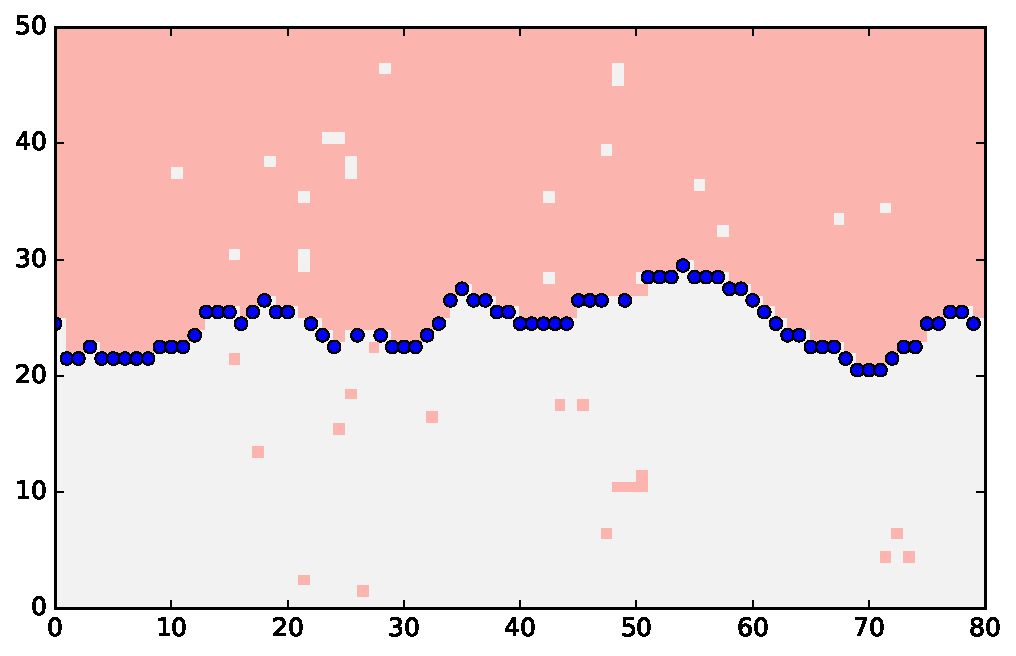
\includegraphics[width=\linewidth]{isingtosos/snap07.pdf}
	\end{minipage}%
	\begin{minipage}[t]{0.5\linewidth}
		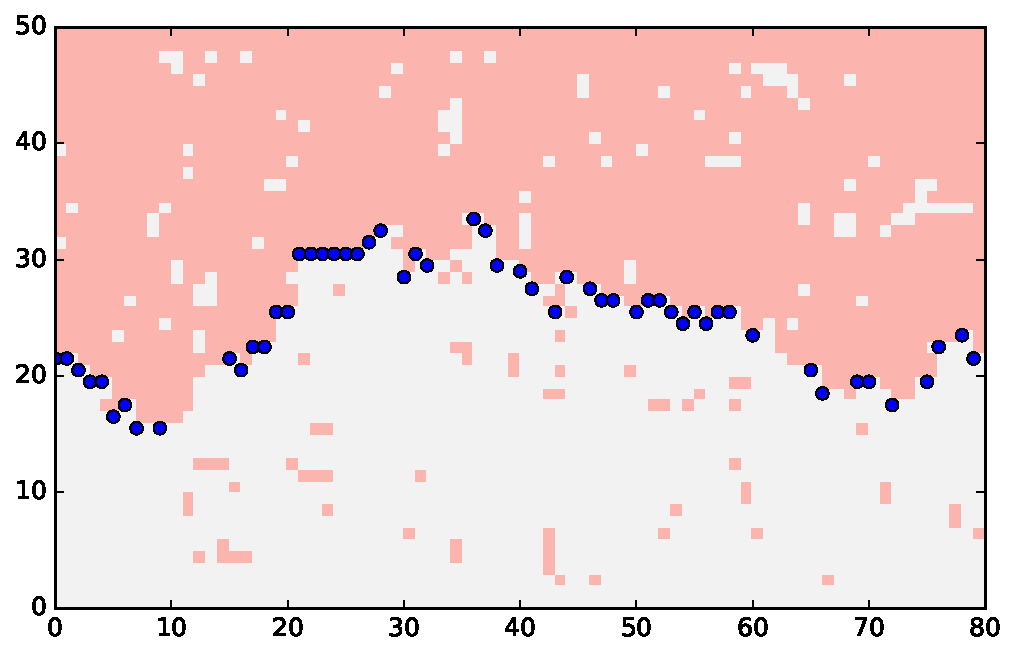
\includegraphics[width=\linewidth]{isingtosos/snap09.pdf}
	\end{minipage}
	\caption{Photo d'un modèle d'Ising pour deux températures différentes($T=0.7 T_C$ et $T=0.95 T_C$ ) avec des conditions périodiques aux bords en X et fixés en Y qui forcent la présence d'une interface entre les phases $+$ (rose) et $-$ (blanc) du système. Plus la température est élevée et plus l'interface fluctue, jusqu'à cesser d'exister pour $T \greater T_C$. }
	\label{amas-fixe}
\end{figure}  

Nous rappelons l'Hamiltonien \ref{hamil-mean-field} du champ moyen 
\begin{align}
    H[\phi] = \int d \mx  \frac{\kappa}{2}[{\boldsymbol \nabla} \phi]^2 + V(\phi)
\end{align}
où $V(\phi)$ est un potentiel de possédant deux minima en $\phi_C = \pm1$. On considère maintenant que le champ sur les sites de notre réseau est égal à $\pm \phi_C = \pm 1$. On note ${\bf i}:=(x,y,z)$ le site du réseau correspondant aux coordonnées $(x,y,z)$. Sur un réseau carré discret de pas $a=1$, la discrétisation du premier terme au premier ordre se traduit par 
\begin{align}
    [{\boldsymbol \nabla} \phi({\bf i})]^2 &= \left( \frac{\partial \phi({\bf i})}{\partial x} \right)^2  + \left( \frac{\partial \phi({\bf i})}{\partial y} \right)^2 + \left( \frac{\partial \phi({\bf i})}{\partial z} \right)^2\nn
    &= (\phi(x,y,z)-\phi(x+1,y,z))^2 + (\phi(x,y,z)-\phi(x,y+1,z))^2 + (\phi(x,y,z)-\phi(x,y,z+1))^2 \nn
    &= 2 (1-\phi(x,y,z)\phi(x+1,y,z) + 2 (1-\phi(x,y,z)\phi(x,y+1,z) +2 (1-\phi(x,y,z)\phi(x,y,z+1) 
    \label{discretisation-landau}
\end{align}
Notons $\sigma_i = \phi({\bf i}) = \pm 1$, et $J := \kappa$. On obtient alors l'Hamiltonien du modèle d'Ising
\begin{equation}
	\mH =  - \sum_{<i j >} J \sigma_i \sigma_j + \frac{V(\sigma_i)+V(\sigma_j)}{2}
	\label{hamil-ising}
\end{equation}
où $\sum_{< ij >}$ est une somme sur toutes les paires de premiers voisins. Le champ externe $V(i)$ a ici été symmétrisé et le terme constant de \ref{discretisation-landau} a été retiré.
Le modèle d'Ising\cite{niss_history_2005,niss_history_2009} est donc un modèle sur réseau à interactions courtes entre les particules. Puisque les constituants $\sigma_i$ du système sont tous égaux à $\pm!$, on appelle ce système un système de spin sur réseau. Dans le cas où la variable $\sigma_i$ est continue, on parle de modèle XY. Pour plus de généralité, il est également possible de varier l'interaction entre les plus proches voisins en posant $J = J_{ij}$. Si $ J_{ij} =0$, on parle d'interaction ferromagnétique favorisant à homogénéiser le système malgré l'agitation thermique. Si  $J_{ij} < 0$, on parle d'interaction antiferromagnétique favorise les systèmes où chaque spin possède un signe différent de celui de tous ses plus proches voisins. On prendra pour le reste de cette thèse $J=1$.

Ce modèle décrit précisément les transitions de phases dans les matériaux magnétiques uniaxiaux \cite{de_jongh_experiments_1974,wp_wold_ising_2000,ikeda_neutron_nodate}. Il est par ailleurs le modèle le plus simple à l'intérieur de sa classe d'universalité, qui contient également les transitions liquide/gaz ainsi que l'émulsion de liquides binaires. Ce modèle ne possède pas de transitions de phase en une dimension. La solution en deux dimensions a été trouvée par \cite{onsager_crystal_1944}, prouvant l'existant d'une transition de phase à 
\begin{align}
     T_{2D,C} = \frac{2J}{k_B \ln(1 + \sqrt{2})} \simeq 2.27 \frac{J}{k_B}
\end{align}
Puisque ce modèle découle de la discrétisation du champ moyen, ces approches donnent beaucoup d'informations sur la transition de phase et ses propriétés au point critique en 4 dimensions et au-delà, avec $d=4$ étant la dimension critique supérieure. Cependant le modèle n'a pas encore été résolu pour $d=3$, bien que de nombreuses simulations numériques \cite{preis_gpu_2009} ont permis de trouver que la transition critique était à
\begin{align}
    T_{3D,C} \simeq 4.51 \frac{J}{k_B}
\end{align}

En faisant la transformation\cite{goldenfeld_lectures_2018} 
\begin{align}
    n_i =  \frac{\sigma_i +1}{2}
\end{align}
afin que $n_i(\sigma_i = 1) = 1$ et $n_i(\sigma_i = -1) = 0$, on obtient l'Hamiltonien
\begin{equation}
	\mH =  - \sum_{< i j >}  J_{ij} \left( 4 n_i n_j -2 ( n_i+n_j) + 1 \right)+ \sum_{< i j >}  J_{ij} \frac{V(\sigma_i)+V(\sigma_j)}{2}  
\end{equation}
où le terme constant $\sum_{< i j >}  J_{ij}$ ne modifie la fonction de partition $\mZ$ que d'une constante. On définit alors 
\begin{align}
	\mH_{LG} &=  - 4 \sum_{< i j >}  J_{ij}  n_i n_j  + 2 \sum_{< i j >}  J_{ij}  (n_i+n_j) + \sum_{< i j >}  J_{ij} \frac{V(\sigma_i)+V(\sigma_j)}{2}  \nn
       &=  - 4 J \sum_{< i j >}  J n_i n_j  + \mu \sum_i  n_i + \sum_{< i j >}  J \frac{V(\sigma_i)+V(\sigma_j)}{2}  
\end{align}
où l'on a considéré $J_{ij} = J$ constant et définit le potentiel chimique pour les particules liquide-gaz comme $\mu=4Jc$, avec $c$ la connectivité du graphe ($z=2$ en 1D, $z=4$ en 2D et $z=6$ en 3D). Une phase magnétique positive dans le modèle d'Ising s'apparente dès lors à un état de haute densité (un liquide), tandis qu'une phase négative est considérée comme une phase de basse densité, c'est-à-dire un gaz.
Ce modèle représente également un mélange binaire entre deux types de particules $A$ et $B$ comme par exemple un polymère dans un solvant, les particules identiques s'attirent tandis que les particules d'un type différent se repoussent. 
Ici, le potentiel chimique $\mu$ est la variable conjugée au nombre de particules $\sum_i n_i$, tandis que dans les systèmes de spins, le champ magnétique $h$ est la variable conjugée de l'aimantation $\sum_i \sigma_i$.
On peut donc parler d'un champ magnétique uniforme pour un système de spins dans l'ensemble canonique ou de potentiel chimique pour un système de particules dans l'ensemble grand-canonique, et que la physique reste la même. 

%%%%%%%%%%%%%%%%%%%%%%%%%%%%
    \subsection{Charactérisation de l'interface}
%%%%%%%%%%%%%%%%%%%%%%%%%%%%

L'étude de l'interface entre les phases $+$ et $-$ nécessite la brisure de la symétrie de translation au sein du système. Cela peut se réaliser via des conditions aux bords non-périodiques dans la direction $z$, soit avec des conditions aux bords fixes avec $\sigma(z=0) = -1$ et $\sigma(z=L)=+1$, soit en favorisant les spins sur les rangées du bords grâce à l'ajout d'un potentiel $V(z) = h (\delta(z)-\delta(z-L))$.
Une interface se charactérise par sa position moyenne et sa largeur. La manière la plus simple de mesurer ces charactéristiques est de comparer le profil de magnétisation \cite{stecki_magnetization_1994}  dans l'axe $z$ perpendiculaire à l'interface
\begin{align}
    m(z) = \frac{1}{L'^2} < \sum_{xy} \sigma(x,y,z) >
\end{align}
aux résultats de champ moyen \ref{kink}. Le fit nous donne alors la position moyenne et la largeur de l'interface. La largeur de l'interface est définie comme le déplacement moyen autour de la moyenne, c'est-à-dire
\begin{align}
    w^2 = <h^2>-<h>^2
\end{align}
où $h$ est la position de l'interface. On trouve alors que la largeur de l'interface est égale à
\begin{align}
    w^2 = 2 \frac{ \int_0^L dz z \frac{d m(z)}{dz}}{\int_0^L dz \frac{d m(z)}{dz}}
\end{align}
 
On définit maintenant la tension superficielle de l'interface comme la différence entre l'énergie libre en absence d'interface avec l'énergie libre de l'interface \cite{abraham_transfer_1973,abraham_interface_1976,richards_numerical_1993}, c'est-à-dire
\begin{align}
    \sigma &= \lim_{L',L \to \infty} \frac{1}{L'^2} \ln \left( \frac{Z^{+-}}{Z^{++}} \right) 
\end{align}
où $Z^{+-}$ est la fonciton de partition du système avec des conditions aux bords $(+-)$ et $Z^{++}$ la fonction de partition avec des conditions aux bords $Z^{++}$.
Par diagonalisation de la matrice de transfert du système (que nous introduirons plus tard), en absence de champ externe, nous obtenons la tension superficielle
\begin{align}
    \sigma = 2 \beta J + \log(\tanh(\beta J))    
\end{align}

%%%%%%%%%%%%%%%%%%%%%%%%%%%%
    \subsection{Méthode de calcul de la force de Casimir}
%%%%%%%%%%%%%%%%%%%%%%%%%%%%

\begin{figure}
	\begin{minipage}[t]{0.32\linewidth}
		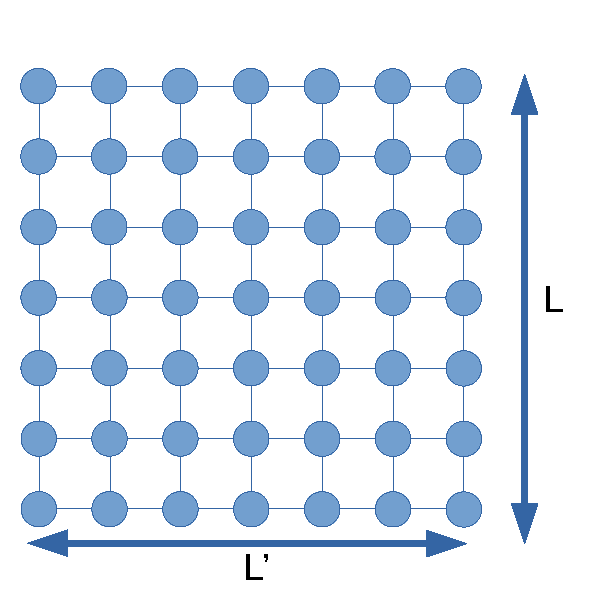
\includegraphics[width=\linewidth]{isingtosos/cross-h0.pdf}
		\caption*{$\mH_0$}
	\end{minipage}
	\begin{minipage}[t]{0.32\linewidth}
		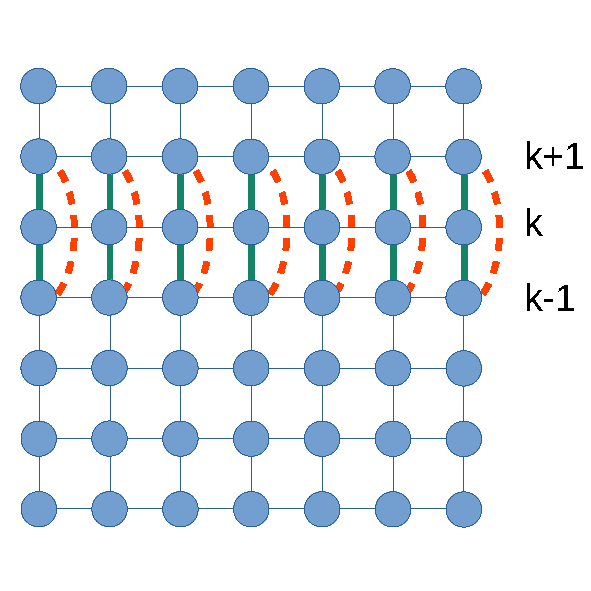
\includegraphics[width=\linewidth]{isingtosos/cross-hlambda.pdf}
		\caption*{$\mH(\lambda)$}		
	\end{minipage}
	\centering
	\begin{minipage}[t]{0.32\linewidth}
		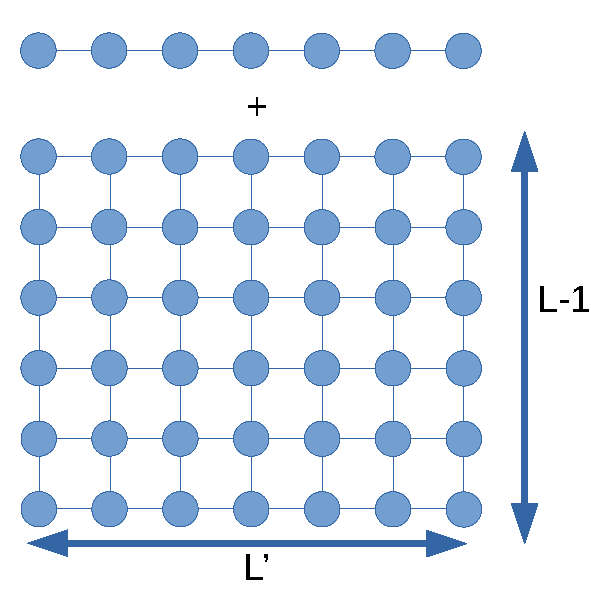
\includegraphics[width=\linewidth]{isingtosos/cross-h1.pdf}
		\caption*{$\mH_1$}
	\end{minipage}
	\caption{Découplage progressif de la $k$-ième couche du système afin de calculer la variation de l'énergie libre grâce à l'Hamiltonien de transition. Les liens en bleu ont une énergie de $\beta J$, les liens en rouge une énergie de $\lambda \beta J $ et les liens en vert une énergie de $ (1-\lambda) \beta J$. Reproduction 2D de \cite{vasilyev_monte_2007}.}
	\label{decouplage}
\end{figure}

Comme vu dans la section \ref{sec-casimir}, on retrouve dans l'énergie libre du système toute l'information nécessaire sur les effets de taille finie, principalement la force de Casimir critique. L'énergie libre ne peut être exprimée par des moyennes d'observables facilement calculables dans les simulations de Monte Carlo. La force de Casimir étant 
\begin{align}
    F(t,h,L) = - \frac{\partial \Omega}{\partial L}
\end{align}
on remarque que le calcul seul de la dérivée par rapport à la hauteur $L$ du systèème est suffisant. Pour se faire, Vasilyec \cite{vasilyev_monte_2007} a développé une méthode pour calculer sa dérivée vis-à-vis d'un paramètre fictif de couplage. Bien que la taille d'un ystème sur réseau soit discrète, il est possible d'obtenir une taille continue du réseau grâce au découplage progressif d'une couche du système. 
Si $\mH_0$ est l'Hamiltonien du système de hauteur $L$ et $\mH_1$ l'Hamiltonien de hauteur $L-1$ (voir figure \ref{decouplage}), alors on pose l'Hamiltonien de transition
\begin{align}
    H_{tr}(\lambda) = (1-\lambda) H_0 + \lambda H_1
    \label{hamil-trans}
\end{align}
avec $\lambda \in [0,1]$, et qui interpole $H_0$ et $H_1$ lorsque $\lambda$ va de $0$ à $1$. 
L'Hamiltonien de transition $H_{tr}(\lambda)$ dépend également de la position $k_0 \in {1,2,...,L}$ (selon la direction $z$ de la couche qui se découple du reste du système en fonction de $\lambda$, c'est-à-dire de \ref{decouplage}(a) à \ref{decouplage}(c). L'Hamiltonien résultant est charactérisé par les constantes de couplage décrites dans la figure \ref{decouplage}(b). L'énergie libre associée à cet Hamiltonien est
\begin{align}
    \Omega_{tr}(\lambda) = -k_B T \ln \left( \sum_{h_1 ... h_L} \exp(-\beta H_{tr}(\lambda)) \right)
\end{align}
De la dérivée de l'énergie libre découle
\begin{align}
    \frac{\Omega_{tr}(\lambda)}{d\lambda} = < \mH_1 - H_0>_{H_{tr}(\lambda)}
\end{align}
où $< \cdot >_{\mH_{tr}(\lambda)}$ représente la moyenne statistique sur le système en transition, facilement calculable dans les simulations numériques. En intégrant sur le couplage, on trouve que
\begin{align}
    \Omega_1 - \Omega_0 = \int_0^1 d\lambda  < H_1 - H_0>_{\mH_{tr}(\lambda)}
\end{align}
Finalement, dans la limite où l'épaisseur du système est suffisament grande pour que la variation d'une couche soit suffisement petite ($L' \gg 1$), on trouve que
\begin{align}
   - \frac{\partial \Omega(t,h,L)}{\partial L} \simeq  \int_0^1 d\lambda  < \mH_1 - \mH_0>_{\mH_{tr}(\lambda)}
\end{align}
Bien que $H_{tr}(\lambda)$ dépende de la rangée $k_0$ que l'on a décidé de découpler, et par transition $H_1-H_0$ et $< H_1 - H_0>_{\mH_{tr}(\lambda)}$, l'intégrale $\int_0^1 d\lambda < H_1 - H_0>_{\mH_{tr}(\lambda)}$ est indépendante de ce choix tant que les conditions aux borrds ne sont pas affectés par l'extraction de la couche $k_0$. 	

{\color{red} rajouter quelques résultats sur la forme de la force de Casimir $+-$? }

%%%%%%%%%%%%%%%%%%%%%%%%%%%%%%%		
    \section{Modèle Solid-On-Solid}
%%%%%%%%%%%%%%%%%%%%%%%%%%%%%%%  
%%%%%%%%%%%%%%%%%%%%%%%%%%%%%%%  
    \subsection{Définition du modèle}
%%%%%%%%%%%%%%%%%%%%%%%%%%%%%%%  
Le modèle d'Ising permet d'étudier de nombreux systèmes différents, que ce soit pour les propriétés de bulk, la dynamique de coarsening ou les propriétés de l'interface. Dans ce dernier cas, il n'est pas nécessaire de posséder toutes les informations sur le bulk afin d'obtenir les propriétés de l'interface. 
Tout comme on est passés des équations de champ moyen du modèle A et B aux équations d0interface Edwards-Wilkinson, le passage d'un système entier à l'étude spécifique de l'interface peut se faire dans les modèles sur réseau.
À très basse température, les interfaces sont bien délimitées et il y a très peu de clusters de la phase $+$ dans la phase $-$, et vice-versa. En considérant le système très peu mélangé, il est possible de définir la présence d'une phase par rapport à la hauteur $h_i$ de l'interface. Chaque site prend alors la valeur
\begin{align*}
	\sigma_{i,j} = \sgn(h_i-j)
\end{align*}
où la fonction $\sgn(x)$ est égale à $+1$ si $x >0$ et à $-1$ sinon. Cela revient à considérer que l'énergie d'interaction $J_z$ dans l'axe perpendiculaire à l'interface est bien supérieure à l'énergie d'interaction perpendiculaire à l'interface.

\begin{figure}
	\centering
	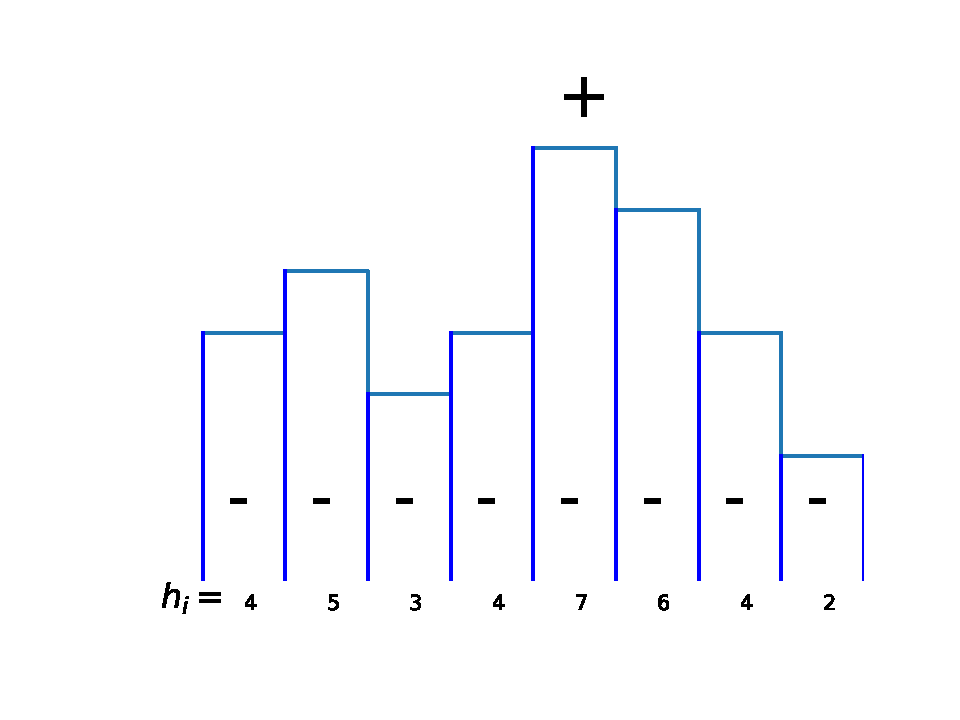
\includegraphics[scale=1]{isingtosos/sos-indiscernable.pdf}
	\caption{Une configuration possible de modèle SOS. Dans la i-ème colonne le bord horizontal de l'interface passe à la hauteur $h_i$. Toutes les particules au-dessus de l'interface sont des spins positifs, et négatifs en dessous. La représentation classique du modèle SOS diffère de ce schéma par l'hypothèse que les particules sont discernables (voir Chapitre \ref{chap-pop}).
	{\color{red} David : pourquoi tu veux mettre cette figure dans un autre chapitre ??}}
    \label{figure-sos}
\end{figure}

En utilisant les identités
\begin{align}
     \min(a,b) &= \frac{|a+b| - |a-b|}{2} \\
    \max(a,b) &=    \frac{|a+b| + |a-b|}{2}
\end{align}
on a
\begin{align}
    \sum_{j=0}^L \sgn(h-j)\sgn(h'-j) = L - 2 |h-h'|
\end{align}
Pour un système d'Ising en deux dimensions de taille $L'\times L$, l'Hamiltonien du modèle d'Ising \ref{hamil-ising}, se réécrit comme 
\begin{align}
    H = 2 J L' (1-L) +2 J \sum_{i=0}^{L'} |h_i-h_{i+1}| + \sum_{i=0}^{L'} V(h_i)
    \label{energie-sos-ising}
\end{align}
où la somme se fait maintenant sur les sites $i$ de hauteur $h_i$ (voir figure \ref{figure-sos}), et le résultat a été divisé par deux pour ne pas compter deux fois les mêmes liens, et 
\begin{align}
    V(h_i) = \sum_{j=0}^L V(\sgn(h-j))
\end{align}
On pose $h_{L'}=h_0$ comme conditions périodiques aux bords.
On peut également calculer directement l'énergie d'un tel système depuis une configuration Solid-On-Solid. Il existe $ L_Y$ liens verticaux par colonne, dont tous sauf un ont une énergie de $-J$, et le lien passant à travers l'interface ayant une énergie de $+J$. L'énergie totale des liens verticaux est donc de $E_y = - J L_X ( L_Y-2)$. De même pour les liens horizontaux, il existe $L_X \times L_Y$ liens au total, dont $\sum_i |h_i-h_{i+1}|$ liens d'énergie $+J$, ce qui nous donne une énergie d'interaction horizontale de $E_x = - J L_X L_Y + 2 \sum_i |h_i-h_{i+1}|$. La somme des deux énergies redonne \ref{energie-sos-ising}.

Le terme $|h_i-h_{i+1}|$ représente la surface de contact horizontale entre les deux phases qui dépend directement de la hauteur, tandis que le terme constant représente la surface de contact verticale.
En simplifiant $2 J = J$ et en retirant l'énergie de volume qui est constante, nous obtenons l'hamiltonien du \textbf{modèle Solid-On-Solid} (SOS)
\begin{align}
    H = J \sum_{i=0}^{L'} |h_i-h_{i+1}| + \frac{V(h_i)+V(h_{i+1})}{2}
    \label{hamil-sos}
\end{align}
où l'on a symmétrisé le potentiel $V(h)$.
Dans le langage liquide/gaz utilisé précédement dans le modèle d'Ising, on peut interpréter la hauteur $h_i$ comme étant le nombre de particules au site $i$, avec les sites au-dessus de l'interface étant considérés comme vides. Lorsque le site $i$ augmente d'une unité, on peut considérer qu'une particule s'est ajoutée au système, et qu'elle s'est évaporée si $h_i$ décroit d'une unité. 

La croissance des cristaux a été le premier système sur lequel le modèle SOS a été développé en 1972 \cite{gilmer_simulation_1972}. Depuis, le modèle a été utilisé pour des systèmes de croissances de cristaux \cite{elwenspoek_kinetic_1987}, a été trouvé en accord avec les expériences de croissance épitaxiale \cite{wilby_scaling_1992}, ou dans le cas des membranes de polymères \cite{gompper_steric_1989}.

Dans le modèle SOS, les $h_i$ peuvent prendre n'importe quelle valeur en tre $0$ et $L$. Une variante de ce modèle est celui où la hauteur $h_{i+1}$ est restreinte uniquement aux valeurs comprises dans $[h_i-a,h_i+a]$. La version du modèle où $a=1$ est appelé le modèle Solid-On-Solid Restreint (RSOS)\cite{privman_transfer-matrix_1989}. Ce modèle est une approximation du modèle SOS à très basse température.  Dans ces conditions, l'interface est très lisse puisque l'on contraint les modes excités de l'interface \cite{kim_conserved_1994,vaysburd_critical_1995}. 

Un modèle qui est plus proche des modèles continus comme l'Hamiltonien \ref{heff} possède une l'interaction gaussienne
\begin{align}
    H = J \sum_{i=0}^{L'} (h_i-h_{i+1})^2 + \frac{V(h_i)+V(h_{i+1})}{2}
    \label{hamil-gsos}
\end{align}
qui possède également une versione restreinte. Le modèle SOS possède, quelque soit l'exposant de l'interaction, une relation étroite avec le modèle $XY$ \cite{knops_exact_1977}.

La dimensionalité du système a été réduite en ne prenant en compte que la hauteur $h_i$ au site $i$ à la place de la position de toutes les particules. L'approximation du modèle SOS implique que les configurations sont analogues à celles d'un mouvement brownien partiellement dirigé auto-évitant. Cette analogie a permis de diagonaliser complètement la fonction de partition dans le cas où il existe un champ magnétique et un potentiel confinant l'interface (nous y reviendrons au paragraphe \ref{par-stab}) \cite{owczarek_exact_1993} et d'étudier les statistiques des déviations extrêmes de l'interface \cite{majumdar_airy_2005,schehr_universal_2006}.

%%%%%%%%%%%%%%%%%%%%%%%%%%%%%%%%%%%%%%%%%%%
	\subsection{Ensemble grand-canonique et potentiel chimique}
	\label{subsec-c-gc}
%%%%%%%%%%%%%%%%%%%%%%%%%%%%%%%%%%%%%%%%%%%

Dans l'ensemble grand-canonique, le nombre de particules dans le système varie, dépendant du potentiel chimique vis-à-vis du réservoir dans lequel il est inséré, ce qui permet à l'interface de bouger librement. Lorsque l'on se place dans l'ensemble canonique, le nombre de particules $N$ sous l'interface est fixe, ce qui introduit une contrainte dans la fonction de partition
\begin{align}
	 Z(N) = \sum_{h_0 h_1 ... h_{L'}} \exp(- \beta \sum_{i} H(h_i,h_{i+1}))  \delta_{\sum_i h_i, N}
	 \label{hamil-sos-cano}
\end{align}
La position moyenne de l'interface est maintenant imposée, ce qui interdit certains microétats, et change les propriétés thermodynamiques de la matrice de transfert comme la distribution des hauteurs de l'interface \cite{siegert_scaling_1993}, même si la moyenne reste la même. Malheureusement, il est impossible de réécrire la contrainte dans le langage des matrices de transfert, empêchant ainsi de calculer analytiquement les différences entre les deux ensembles pour une taille donnée. Il est possible de construire la fonction de partition \textit{ab initio}, mais le grand nombre de sites et de hauteurs permises dans un système classique empêchent le calcul dans un temps CPU raisonnable. 

La fonction de partition \ref{hamil-sos-cano} est en relation vis-à-vis de l'ensemble grand-canonique grâce  au potentiel chimique $\mu$ par
\begin{align}
	 \Xi(\mu) = \sum_N Z(N) \exp((\beta \mu N)
\end{align}
La grande fonction de partition peut s'écrire comme
\begin{align}
    \Xi = \sum_{h_0 h_1 ... h_{L'}}  \exp(-\beta H_{eff}(h_0,h_1,...,h_{L'})
\end{align}
où 
\begin{align}
    H_{eff} = J \sum_{i=0}^{L'} |h_i-h_{i+1}|+ \sum_{i=0}^{L'} V(h_i)-\mu h_i
\end{align}
et de matrice de transfert
\begin{align}
    T(h,h') = \exp\left(-\beta (J |h-h'| - \mu \frac{h+h'}{2} + \frac{V(h)+V(h')}{2} \right)
    \label{tm-sos-grand-cano}
\end{align}

Dans la figure \ref{hauteur-mu}, on montre le nombre moyen de particules par site en fonction du potentiel chimique, pour différentes hauteurs maximales $L$. Ce potentiel chimique simule une pression externe imposée, qui peut soit confiner l'interface vers $h=0$ si $\mu \less 0$ (comme sur la figure), ou le confiner vers $h=L$ si $\mu \greater 0$. 
Ainsi, l'équivalence des ensembles canonique et grand-canonique dans la limite thermodynamique à $\mu$ fixé n'est valable que lorsque le nombre de particules du système canonique $N$ est égal au nombre de particules dans l'ensemble grand-canonique.
\begin{figure}
    \centering
	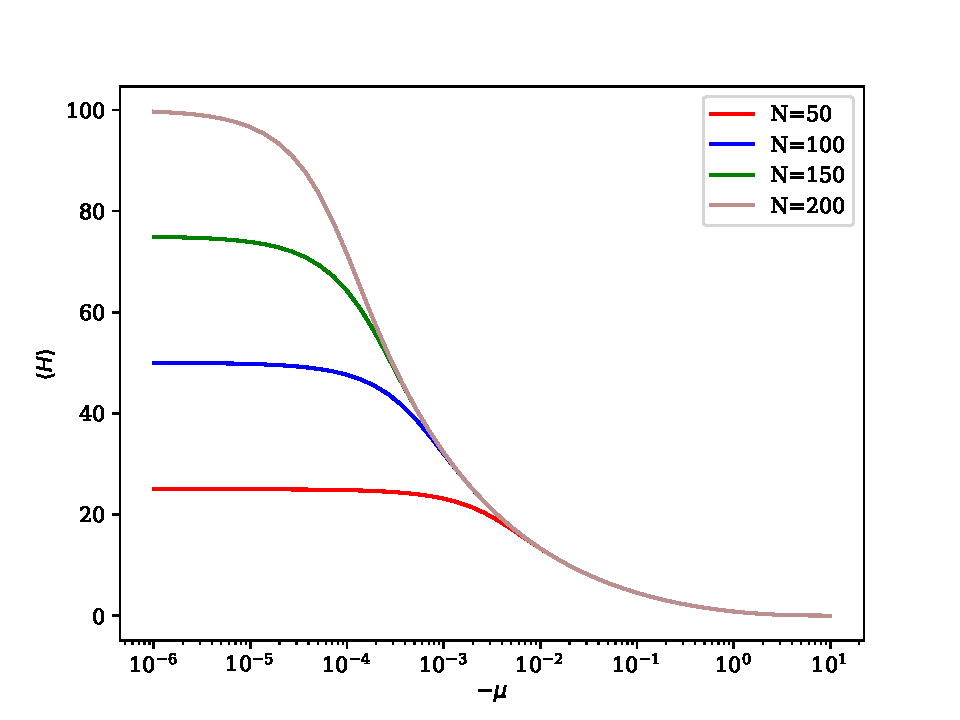
\includegraphics[width=0.7\linewidth]{isingtosos/hauteur-tm-sos.pdf}
	\caption{Position d'équilibre de l'interface \ref{tm-sos-grand-cano} en fonction de $- \mu$ via diagonalisation de la matrice de transfert \ref{tm-sos-grand-cano}. Lorsque le potentiel chimique est trop faible, l'interface est délocalisée et se retrouve à la position $\frac{N}{2}$. }
	\label{hauteur-mu}
\end{figure}

Comme dans le modèle d'Ising, il existe une bijection entre l'usage d'un champ magnétique conjugé à une aimantation par site et l'usage d'un potentiel chimique conjugué à une densité de particules. Nous parlerons donc sans ambigüité de potentiel chimique pour tout potentiel $V(h_i)$ que nous étudierons plus tard, ainsi que de densité de particules $M$.
%%%%%%%%%%%%%%%%%%%%%%%%%%%%%%%%%%%%%%%
  \subsection{Matrice de Transfert}
%%%%%%%%%%%%%%%%%%%%%%%%%%%%%%%%%%%%%%%

	De manière plus générale, l'Hamiltonien d'un système avec des interactions entre les particules peut se réécrire comme $H = \sum_{< ij >} H(h_i,h_j)$ avec
\begin{align*}
  H = \sum_{i=0}^{L'} f(h_i,h_{i+1}) + V(h_i,h_{i+1}) 
\end{align*}
où $f(h_i,h_j)$ est l'énergie d'interaction entre plus proches voisins et $V(h_i,h_j)=\frac{V(h_i)+V(h_j)}{2}$ le potentiel symmétrisé. Pour un système possédant $L'$ sites pouvant continr des valeurs dans $[0,L]$, la fonction de partition de notre système s'écrit 

\begin{align}
 Z = \sum_{h_1=0}^{L} \sum_{h_2=0}^{L}... \sum_{h_{L'}=0}^{L¡} \exp(- \beta \sum_{i=0}^{L'} H(h_i,h_{i+1}))
   = \sum_{h_1 h_2 ... h_{L'}} \prod_{i=_0}^{L'} \exp(-\beta H(h_i,h_{i+1}))
\end{align}

La matrice 
\begin{align}
    T(h_i,h_j) = e^{-\beta H(h_i,h_j)}
    \label{matric-transfert}
\end{align}
est appelée matrice de transfert. On a représenté dans la figure \ref{mat-inf} une matrice infinie correspond à la limite thermodynamique dans le cas où les sites peuvent prendre n'importe quelle valeur dans $[-\infty,\infty]$, qui correspond au cas où l'interface est centrée en $h=0$ et ne possède pas de conditions aux bords. Lorsqu'il s'agit de diagonaliser cette matrice infine numériquement, il suffit de faire la translation $h_i \to h_i - \frac{L}{2}$, où $L$ est la taille de la matrice de transfert, tendant vers l'infini.

Puisque le système est périodique (c'est-à-dire que $h_{L+1} = h_1$),  la matrice est périodique également, c'est-à-dire que $T(h_L,h_{L+1}) = T(h_L,h_1)$ \cite{pearce_exact_1989}, et elle est également symétrique, La matrice de transfert peut donc être diagonalisée, nous écrivons ses vecteurs valeurs propres comme
\begin{align}
    T | \lambda> = \lambda |\lambda>
\end{align}
Ces vecteurs propres sont également orthonormaux 
\begin{align}
    < \lambda | \lambda'> = \delta_{\lambda \lambda'}
\end{align}
On note par $\lambda_0$ la plus grande valeur propre de T, par $\lambda_1$ la deuxième plus grande valeur propre etainsi de suite. 
Ainsi on peut diagonaliser la fonction de partition par la trace de la matrice de transfert \cite{abraham_transfer_1973}
\begin{align}
  Z = \sum_{h_1 h_2 ... h_{L'}} \prod_{i} T(h_i,h_{i+i}) = Tr( T^{L'})  = \sum_\lambda <\lambda | T^{L'} | \lambda> = \sum_\lambda \lambda^{L'}
  \label{partition-trace-lambda}
\end{align}

\begin{figure}
    \begin{align}
    T = \begin{bmatrix} 
            \ddots & \vdots & \reflectbox{$\ddots$} \\ 
            e^{-\beta H(-1,-1)} &  e^{-\beta H(-1,0)} & e^{-\beta H(1,-1)} \\
            \dots & e^{-\beta H(0,0)} & \dots  \\
            e^{-\beta H(1,-1)} & e^{-\beta H(1,0)} & e^{-\beta H(1,1)}   \\ 
             \reflectbox{$\ddots$} & \vdots &\ddots  \\ 
        \end{bmatrix}
    \end{align}
    \caption{Matrice de transfert infinie et symmétrique \ref{matric-transfert}.}
    \label{mat-inf}
\end{figure}

Dans la limite thermodynamique $L' \to \infty$, seul le plus grand vecteur propre est relevant, puisque la fonction de partition devient
\begin{align}
    Z(L\to \infty) \simeq \lambda_0^{L'}
\end{align}
Nous trouvons alors que l'énergie libre par site est égale à 
\begin{align}
	F =  - \frac{1}{L' \beta} \ln(Z) \simeq - \frac{1}{\beta } \ln( \lambda_0)
	\label{energie-libre-site}
\end{align}
Dans la figure \ref{fig-thermo-libre} on montre l'évolution de l'énergie libre par site $F(L')$ dans le cas d'un potentiel nul.On détermine alors que l'approximation de la limite thermodynamique est vraie pour $L' \greater 150 $.
\begin{figure}
    \centering
	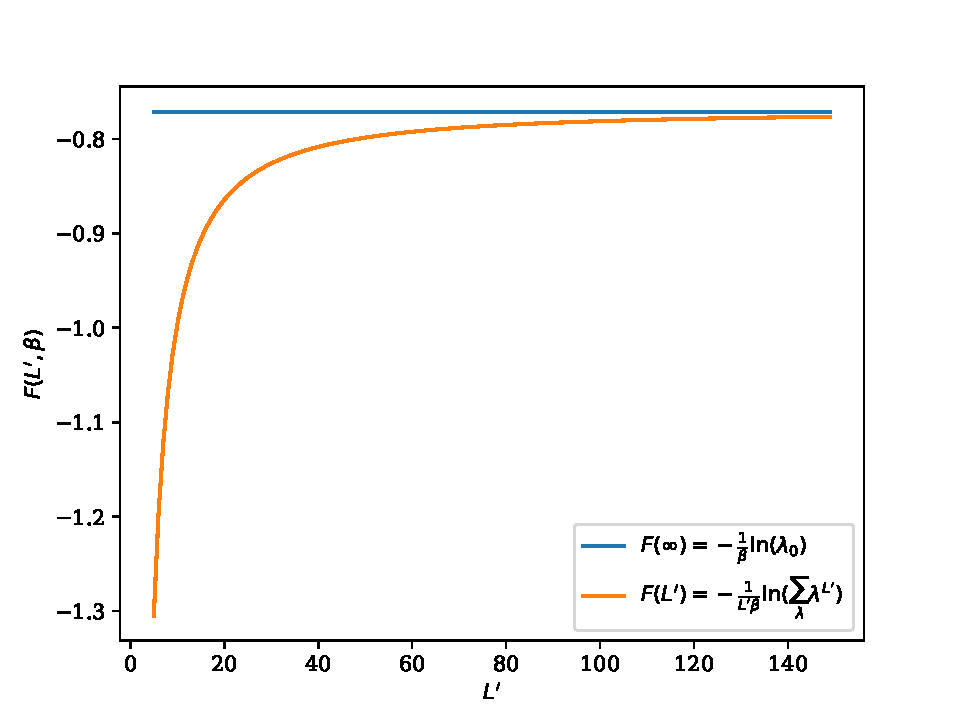
\includegraphics[width=0.7\linewidth]{isingtosos/freeene-thermo-libre.pdf}
	\caption{Énergie libre par site $F(L')$ en fonction du nombre de sites $L'$ comparé à la limite thermodynamique $F(\infty)$, pour un système de hauteur $L=100$, $\beta=1$, $J=1$ et $V(h_i)=0$.}
	\label{fig-thermo-libre}
	\vspace{-0.5cm}
\end{figure}  
Afin de calculer la densité moyenne par site $M$, on introduit la matrice des hauteurs $\hat{M}$ définie par son action sur les vecteurs $|h>$ de la base de la matrice de transfert par
\begin{align}
    <h|\hat{M} |h'> = \delta_{h,h'} h
\end{align}
On trouve alors la densité par site 
\begin{align}
	M = < h > = \frac{1}{L'} \sum_i h_i =  \frac{1}{Z} \sum_\lambda \lambda^{L'} < \lambda | \hat{M} | \lambda > \simeq < \lambda_0 | \hat{M} | \lambda_0 > 
	\label{tm-magnetisation}
\end{align}
On en déduit la variance sur la hauteur par site
\begin{align}
	w^2 = < (h - M)^2 > = \frac{1}{Z} \sum_\lambda \lambda^{L'} < \lambda | \hat{M}^2 | \lambda > - < \lambda | \hat{M}| \lambda >^2  \simeq  < \lambda_0 | \hat{M}^2 | \lambda_0 > - M^2
\end{align}
On peut retrouver ces deux observables en calculant le premier et le second moment de la densité de probabilité qu'un site se trouve à la hauteur $h$
\begin{align}
	p(h) = \frac{1}{Z} \sum_\lambda \lambda^{L'} <\lambda | h >^2 \simeq < \lambda_0 | h >^2
\end{align}
La fonction de corrélation à deux points du système se calcule grâce à la formule
\begin{align}
    C(r) &= < h_i h_{i+r} > - M^2 = \frac{1}{Z} \sum_{\lambda \neq \lambda_0} < \lambda_0 | M | \lambda > < \lambda | M | \lambda_0 > \left( \frac{\lambda}{\lambda_0} \right)^r  
\end{align}
qui devient, dans la limite où $r$ est grand, 
\begin{align}
    C(r) \simeq < \lambda_0 | M | \lambda_1 > < \lambda_1 | M | \lambda_0 > \left( \frac{\lambda_1}{\lambda_0} \right)^r
\end{align}
{\color{red} what did you mean in your corrections by "explain when this is true-what happens to $\lambda_2$ etc" ? }
À grande distance, cette fonciton de corrélation a un charactère exponentiel, ce qui nous permet de définir la longueur de corrélation à grande distance $\xi$
\begin{align}
    \xi = - \frac{1}{\ln(\frac{\lambda_1}{\lambda_0})}
    \label{longueur-correl-thermo}
\end{align}


%%%%%%%%%%%%%%%%%%%%%%%%%%%%%%%%%%%%%
	\subsection{États libres dans un système SOS infini}
	\label{par-stab}
%%%%%%%%%%%%%%%%%%%%%%%%%%%%%%%%%%%%%

Prenons un système de taille $L$ dans la limite thermodynamique $L'\to \infty$. Comme vu précédement, seules les valeurs de la plus grand valeur propre influe sur les propriétés statistiques. Soit 
\begin{align}
    \psi_\lambda(h)= <h|\lambda>
\end{align}
la projection du vecteur propre associé à la valeur propre $\lambda$ de la matrice de transfert sur la base des hauteurs $|h>$ dans un système infini de part et d'autre de l'interface.
Dans la limite $\beta=0$, c'est-à-dire pour une température infinie, tous les termes de la matrice de transfert sont égaux à $1$, menant à des vecteurs propres nuls. Dans ce cas, la densité de probabilité $p(h)$ est nulle pour tout $h$, ce qui signifie qu'il n'existe pas d'interface. Le modèle SOS n'est donc pas valable dans cette limite. De même, pour une température nulle $\beta=\infty$, la matrice de transfert devient la matrice identité. Les valeurs propres deviennent toutes égales à $1$ et les vecteurs propres sont $\psi_i(h) = \delta_{h,i}$ où ici $i$ est l'indice de la i-ème valeur propre $\lambda_i = 1$. La probabilité de trouver l'interface à la hauteur $h$ devient $p(h) = \frac{1}{Z}\sum_{i} <\lambda_i | h >^2 = 1$. La température nulle a pour effet de geler l'interface sur une seule hauteur, même si toutes les hauteurs sont équiprobables. Bien que les micro-états soient extrêmement différents pour une température finie, les propriétés macroscopiques sont identiques à cause du même poids statistique associé à chaque état.

Pour une température finie et en absence de potentiel\cite{guyer_sine-gordon_1979,chui_pinning_1981}, l'équation du vecteur propre donne
\begin{align}
	\sum_{h=-\infty}^\infty T(h,h') \psi_\lambda(h) = \lambda \psi_\lambda(h')
\end{align}
En introduisant l'ansatz $\psi_\lambda(h) = \alpha_{\lambda}^h$ et en séparant de la somme les termes pour $h$ négatifs et positifs, on trouve aisément que 
\begin{align}
	\lambda = \frac{\sinh(\beta J)}{\cosh(\beta J)-(\alpha_{\lambda}+\alpha_{\lambda}^{-1})} 
\end{align}
Dans la limite thermodynamique, la probabilité de présence de l'interface à la hauteur $h$ est $p(h) = <\lambda_0|h>^2 = |\psi_0(h)|^2$. Le système ne possédant aucune brisure de symétrie particulière, la probabilité $p(h)$ est finie pour tout $h$ avec $p(h)=p(-h)$. Dès lors, l'ansatz supposé $\psi_\lambda(h) = \alpha_{\lambda}^h$ implique que $\alpha_{\lambda}$ soit de la forme $e^{ik}$ où $k$ est la longueur d'onde associée à la valeur propre $\lambda$. On obtient que 
\begin{align}
	\psi_k(h) =& e^{ikh} \\
	\lambda =& \frac{\sinh(\beta J)}{\cosh(\beta J) - \cos(k)}
	\label{lambda-sos}
\end{align}

L'existence d'une solution de ce genre indique que l'interface n'est pas localisée dans le cas d'un système infini (ou semi-infini) en absence de tout potentiel, ce qui conduit à de nombreux problèmes numériques. 

Une manière simple de localiser l'interface est de rajouter un potentiel $V(h) = -B \delta_{h,0}$ \cite{chui_pinning_1999,chalker_pinning_1981,chalker_pinning_1982}, qui augmente la probabilité de présence de l'interface à $h=0$. La recherche d'un état localisé nous donne un ansatz de la forme 
\begin{align}
	\psi_\lambda(h) = \begin{cases} |\alpha|^h & \text{si } h \neq 0 \\ \psi_{\lambda,0} & \text{sinon} \end{cases} 
\end{align}
L'équation du vecteur propre devient
\begin{align}
	\sum_{h=-\infty}^\infty \exp(\beta |h-h'|- \beta B \delta_{h,0}) \psi_\lambda(h) = \lambda \psi_\lambda(h')
\end{align}
En notant $T(h,h') = R^{|h-h'|}$ pour $h \neq h' \neq 0$,  on obtient la même équation à un signe près dans l'exposant que l'on soit à $h'\greater 0$ ou $h' \greater 0$
\begin{align}
	\left( \frac{R}{\alpha} \right)^{\pm h'} \left[ \psi_{\lambda,0} + \frac{R \alpha}{1 - R \alpha} + \frac{\alpha}{R - \alpha} \right] + \left[ \frac{1}{1-R \alpha} - \frac{R}{R-\alpha} \right] = \lambda
\end{align}
Puisque cette équation est vraie pour tout $h'$, le premier terme doit être nul, ce qui nous donne
\begin{align}
	\psi_{\lambda,0} &= - \frac{\alpha}{R-\alpha}-\frac{R \alpha}{1-R \alpha} \\
	\lambda &= \frac{1}{1-R \alpha} - \frac{R}{R-\alpha}
\end{align}
L'équation du vecteur propre à $h'=0$ nous donne par ailleurs 
\begin{align}
	\psi_{\lambda,0} + 2 \frac{R \alpha}{1-R \alpha} = \lambda \psi_{\lambda,0} e^{-\beta B}
\end{align}
L'existence d'une solution cohérente $\alpha \less 1$ autorise la présence d'une interface localisée grâce à un potentiel dit d'épinglage (\textit{pinning}) \cite{burkhardt_localisation-delocalisation_1981,kroll_solid--solid_1981,kroll_pinning_1982,kroll_interface_1983}.
Dans le cas d'une géométrie semi-infinie, la présence d'un potentiel chimique exerçant une pression sur l'interface permet de la maintenir confinée, comme expliqué dans la section \ref{subsec-c-gc}.

D'autres méthodes existent pour confiner l'interface. Le cisaillement d'une interface diminue sa largeur et permet de la localiser dans l'espace. On peut également proposer deux potentiels chimiques différents pour chaque phase à une hauteur de l'interface prédéfinie, comme le ferait un laser dans un liquie binaire dont chaque phase  a un incident de réfraction différent \cite{casner_laser-induced_2003,delville_laser_2009} (voir chapitre \ref{sec_laser}). Dans un système infini, une autre possibilité est de définir un champ magnétique symétrique rendant plus difficile la présence de l'interface loin de $0$. 

%%%%%%%%%%%%%%%%%%%%%%%%%%%%%%%
\section{Conclusion}
%%%%%%%%%%%%%%%%%%%%%%%%%%%%%%%

La discrétisation sur un réseau carré du champ $\phi(\mx,t)$ mène directement au modèle d'Ising. Ce modèle sur réseau est extrêmement important puisqu'il est appartient à la même classe d'universalité que les ensembles liquide/gaz, les gaz sur réseau ou les liquides binaires. Sa relation étroite avec les théories de champ moyen lui donne de nombreuses méthodes d'approches, comme le groupe de renormalisation, et les simulations numériques de par sa nature discrète. 

L'approximation basse température, dans laquelle on suppose qu'au niveau de l'interfae entre deux phases il n'existe pas d'impueretés, s'appelle le modèle Solid-On-Solid. Ce modèle permet d'étudier les propriétés de l'interface par diagonalisation directe de la matrice de transfert, ou par simulations numériques. 
Pour finir, nous avons montré comment diagonaliser la matrice de transfert dans le cas le plus simple, celui d'un système infini en absence de tout potentiel, et nous avons vu comme dans un tel système, l'interface n'est pas localisée.
